\documentclass{scrartcl}
\usepackage[utf8]{inputenc}
\usepackage[T1]{fontenc}
\usepackage[ngerman]{babel}
\usepackage{amssymb}
\usepackage{amsmath}
\usepackage{algorithmicx}
\usepackage{algpseudocode}
\usepackage{graphicx}
\usepackage{framed}
\usepackage{xcolor}
\usepackage[nottoc]{tocbibind}
\usepackage{caption}
\usepackage{setspace}
\onehalfspacing

\colorlet{shadecolor}{gray!25}
\setlength{\parindent}{0pt}

\newcommand{\abs}[1]{\left\lvert#1\right\rvert}
\newcommand{\R}{\mathbb{R}}

\begin{document}

\title{Lösen des Poisson-Problems mittels Finite-Differenzen-Diskretisierung}
\author{Marisa Breßler und Anne Jeschke}
\date{29.11.2019}
\maketitle

\tableofcontents

\pagebreak
\section{Einleitung}
Die vorliegende Arbeit befasst sich mit dem numerischen Lösen des Poisson-Problems mittels Finite-Differenzen-Diskretisierung. Die Methode greift auf das numerische Ableiten via finiter Differenzen zurück, welches wir in unserem Bericht vom 08.11.2019 vorgestellt und untersucht haben.\\
In der Wissenschaft wird man häufig mit (partiellen) Differentialgleichungen konfrontiert. Eine analytische Lösung derselben gestaltet sich in vielen Fällen schwierig oder ist gar nicht möglich. Ein wichtiges Beispiel auf diesem Gebiet ist die Poisson-Gleichung. Diese kommt bei der Beschreibung vieler physikalischer Phänomene zur Anwendung, so beispielsweise in der Elektrodynamik oder bei mechanischen Prozessen. Nachfolgend sollen einige konkrete Beispiele aufgezählt werden:
\begin{itemize}
\item elektrostatisches Potential $u$ zu einer gegebenen Ladungsdichte $f$
\item Gravitationspotential $u$ zu einer gegebenen Massendichte $f$
\item Temperaturverteilung $u$ im stationären Zustand bei einer gegebenen Verteilung von Wärmequellen $f$
\item Auslenkung einer gespannten Membran oder Saite, die einer äußeren Belastung standhalten muss (Dimension $d=1$)
\item ein Dach unter einer Schneelast o.ä. (Dimension $d=3$)
\end{itemize}
Bereits hier wird deutlich, dass die Poisson-Gleichung Probleme in eine, zwei, drei oder mehr Richtungen beschreiben kann. Durch Diskretisieren der Problemstellung und das Abbilden der partiellen Differentialgleichung auf lineare algebraische Gleichungen ist es möglich, das Poisson-Problem näherungsweise (d.h. mit einem gewissen Fehler) zu lösen. Im Speziellen approximiert die Finite-Differenzen-Methode die exakte Lösung auf einem Gitter der Schrittweite $h$. Dazu müssen alle in der partiellen Differentialgleichung auftretenden Funktionswerte und Ableitungen durch finite Ausdrücke ersetzt werden. Wie das möglich ist und wie uns das bei der Lösung des Poisson-Problems helfen kann, wollen wir im Folgenden näher erläutern.\cite{schwedt2016, tischendorf2019}


\pagebreak
\section{Theoretische Grundlagen}
Wir wollen das Poisson-Problem lösen.
Dazu wird ein Gebiet $\Omega\subset\R^d$ ($d\in\mathbb{N}$) und dessen Rand $\partial\Omega$ betrachtet.
Die zwei Funktionen $f\in C(\Omega ; \R)$ und $g\in C(\partial\Omega ; \R)$ sind gegeben.
Das Poisson-Problem besteht in der Suche nach einer Funktion $u$ als Lösung der folgenden elliptischen partiellen Differentialgleichung:
\[\begin{split}
-\Delta u &= f \textrm{ in } \Omega\\
        u &= g \textrm{ auf } \partial\Omega
\end{split}
\]
Hierbei beschreibt $\Delta u$ den Laplace-Operator, der für eine Funktion $u\in C^2(\R^d;\R)$ wie folgt definiert ist: \[\Delta u := \sum_{l=1}^{d} \frac{\partial^2 u}{\partial x^2_l}\]
Für den eindimensionalen Fall, das heißt $d=1$, gilt $\Delta u = u''$. Für höhere Dimensionen $d>1$ beschreibt der Laplace-Operator die Summe aller partiellen Ableitungen von $u$ zweiter Ordnung in jede Richtung der $d$ Dimensionen.

Im Rahmen dieser Arbeit wollen wir uns auf den Fall $\Omega=(0,1)^d$, $d\in\{1, 2, 3\}$ (Einheitsintervall, -quadrat, -würfel) und die Randbedingung $g\equiv0$ konzentrieren, wobei sich unsere Ergebnisse auch auf $d>3$ verallgemeinern lassen.

Um das Problem mit den Mitteln der Numerik zu lösen, diskretisieren wir sowohl das Gebiet $\Omega$, durch eine Auswahl von endlich vielen Punkten $x_1$ bis $x_N$ ($N\in\mathbb{N}$), an denen wir die Funktion $u$ approximieren wollen, als auch den Laplace-Operator, mithilfe der zweiten finiten Differenz, die wir in unserem Bericht vom 08.11.2019 ausführlich vorgestellt haben.
Dies führt schließlich zu einem linearen Gleichungssystem $A^{(d)}\hat{u}=b$.
Die linke Seite der Gleichung entspricht im Wesentlichen dem diskretisierten Laplace-Operator, wobei die Einträge des Vektors $\hat{u}\in\R^N$ die Funktionswerte von $u$ an den $N$ ausgewählten Diskretisierungspunkten approximiert.
Die Einträge des Vektors $b$ sind die bekannten Funktionswerte von $f$ an den $N$ ausgewählten Diskretisierungspunkten, skaliert mit einem Faktor $h^2$.\cite{rheinbach2015, rabus2019}

\subsection{Diskretisierung des Gebietes}
Da wir lediglich endlich viele Punkte auswerten können, müssen wir zunächst das zu untersuchende Gebiet  $\Omega$, diskretisieren.
Nur an diesen bestimmten Stellen können wir die Funktionswerte von $u$ approximieren und folglich das Problem lösen.

Im eindimensionalen Fall teilen wir das Intervall $\Omega=(0,1)$ äquidistant in
$n\in\mathbb{N}$ (mit $n>1$) Teilintervalle der Länge $h:=\frac{1}{n}$ und erhalten somit die $N=n-1$ Diskretisierungspunkte in
$X_1:=\{\frac{j}{n} \: | \: 1\leq j \leq n-1\}$.

Im mehrdimensionalen Fall $d>1$ untersuchen wir analog die Punkte des $d$-fachen kartesischen Produktes dieser Menge $X_d := X_1^d$.
Im zweidimensionalen Fall ergibt sich also das uniforme Gitter $X_2 := X_1^2 = \{(\frac{j}{n}, \frac{k}{n}) \: | \: 1\leq j,k \leq n-1\}$,
im dreidimensionalen Fall $X_3 := X_1^3 = \{(\frac{j}{n}, \frac{k}{n}, \frac{m}{n}) \: | \: 1\leq j,k,m \leq n-1\}$.

Insgesamt erhalten wir in jeder Dimension $(n-1)$, also insgesamt $(n-1)^d$ Diskretisierungspunkte.\cite{rabus2019}

\subsection{Diskretisierung des Laplace-Operators}
Um das Poisson-Problem lösen zu können, müssen wir zudem den Laplace-Operator für $u$ diskretisieren.
Dabei hilft uns die aus dem vorherigen Bericht bekannte Formel für die zweite finite Differenz, die der Approximation der zweiten Ableitung einer Funktion an einer bestimmten Stelle dient.
Im eindimensionalen Fall lautet sie für einen Diskretisierungspunkt $x_i\in X_1$ mit $i \in \{1,...,N\}$:
$D_h^{(2)}u(x_i) = \frac{u(x_i+h) - 2u(x_i)+u(x_i-h)}{h^2}$ und entspricht dem diskreten Laplace-Operator für $u(x_i)$, den wir hier mit $\Delta_h u(x_i)$ bezeichnen.

Im mehrdimensionalen Raum, das heißt für $d>1$, entspricht der diskretisierte Laplace-Operator der Summe der zweiten finiten Differenzen in jede der $d$ Richtungen.
Es sei $e_l$ für $1\leq l \leq d$ der $l$-te Einheitsvektor in $\R^d$. Definiert man die Abbildung $u_{x,l}:\R\to\R$ als $u_{x,l}(t):=u(x+te_l)$, dann kann man die zweite partielle Ableitung von $u$ in Richtung $e_l$ an der Stelle $x$ wie folgt schreiben und mit Hilfe der zweiten finiten Differenz approximieren:
\[\frac{\partial^2 u(x)}{\partial x_l^2} = u''_{x,l}(0) \approx D_h^{(2)}u_{x,l}(0)\]

Dementsprechend definieren wir den diskretisierten Laplace-Operator, die Summe der zweiten finiten Differenzen in jede der $d$ Richtungen, wie folgt:
\[\Delta_h u(x):= \sum_{l=1}^{d} D_h^{(2)}u_{x,l}(0)\]

Nach Diskretisierung des Gebietes gilt mit $h=\frac{1}{n}$ für alle $x\in X_d$, dass $x\pm he_l$ entweder einer der benachbarten Diskretisierungspunkte ist, also $x\pm he_l\in X_d$, oder auf dem Rand des Gebietes $\partial\Omega$ liegt und mit den oben genannten Randbedingungen ($g\equiv0$) $u(x\pm he_l)=g(x\pm he_l)=0$ ist.
Demzufolge können wir den Laplace-Operator von $u$ an der Stelle $x$ mithilfe der Werte von $u$ an den zu $x$ benachbarten Diskretisierungspunkten approximieren.

Für $d=2$ und $x:=(x_1,x_2)\in X_2$ gilt:
\begin{align*}
    -\Delta_h u(x)=\frac{1}{h^2}&(-u(x_1-he_1,x_2)+2u(x_1,x_2)-u(x_1+he_1,x_2)\\
                   &-u(x_1,x_2-he_2)+2u(x_1,x_2)-u(x_1,x_2+he_2))\\
                  =\frac{1}{h^2}&(-u(x_1-he_1,x_2)-u(x_1,x_2-he_2)+4u(x_1,x_2)\\
                   &-u(x_1,x_2+he_2)-u(x_1+he_1,x_2))
\end{align*}

Für $d=3$ steht im Zähler entsprechend der sechsfache Wert von $u(x)$ ($x:=(x_1,x_2, x_3)\in X_3$) und man subtrahiert die Werte der beiden in allen drei Dimensionen benachbarten Punkte. Allgemein ergibt sich folglich die Differenz aus dem $2d$-fachen Wert von $u$ an der Stelle $x \in X_d$ und den sich sternförmig in jede Richtung befindlichen zwei benachbarten Diskretisierungspunkten.\cite{schwedt2016, rabus2019}

\subsection{Aufstellen des linearen Gleichungssystems}
Mit den $N=(n-1)^d$ Diskretisierungspunkten, der Definition des diskretisierten Laplace-Operators über die Formel der zweiten finiten Differenz und den Bedingungen
$-\Delta_h u(x) = f(x) \: \forall x \in \Omega = X_d$,
$u(x) = g(x) = 0 \: \forall x \in \partial\Omega$
erhalten wir $N$ lineare Gleichungen mit $N$ Unbekannten.
Diese wollen wir in die Form eines linearen Gleichungssystems bringen, das die folgende Struktur aufweist: $A^{(d)}\hat{u}=b$.
Dabei sind die Einträge des Vektors $\hat{u}\in\R^n$ die gesuchten Werte der Funktion $u$ an den $N$ Diskretisierungspunkten und die Einträge des Vektors $b$ die gegebenen Funktionswerte von $f$ an den $N$ ausgewählten Diskretisierungspunkten, multipliziert mit einem Faktor $h^2$, den wir als $\frac{1}{h^2}$ aus den Gleichungen der finiten Differenzen ausgeklammert und schließlich auf die rechte Seite der Gleichungen gebracht haben.

Um die $N$ linearen Gleichungen mit Hilfe eines linearen Gleichungssystem lösen zu können, ist es notwendig, dass wir jedem Diskretisierungspunkt $x \in X_d$ eindeutig eine Nummer $S \in \lbrace1, 2, ..., N\rbrace$ zuordnen. Dazu definieren wir für je zwei Diskretisierungspunkte $x=(x_1, x_2, ..., x_d) \in X_d$ und $y=(y_1, y_2, ..., y_d) \in X_d$ die folgende Ordnungsrelation:
\[x <_X y \iff \sum_{l=1}^d x_l n^l < \sum_{l=1}^d y_l n^l\]

Die Punkte (und damit die Gleichungen) werden dann aufsteigend nach $<_X$ geordnet. Der $m$-te Eintrag des Lösungsvektors $\hat{u}(x)$ ist die Approximation der exakten Lösung $u(x)$ am $m$-ten Diskretisierungspunkt ($m = 1, 2, ..., N$). Diese zeilenweise Nummerierung der Gitterpunkte von links nach rechts (von vorn nach hinten, von unten nach oben) folgt der üblichen lexikographischen Ordnung.\cite{vogt2006}
Die von uns entwickelte bijektive Funktion $idx: \lbrace1, 2, ..., n-1\rbrace^d \to \lbrace1, 2, ..., N\rbrace$ berechnet zu einem Diskretisierungspunkt
$x = (\frac{j_1}{n}, \frac{j_2}{n}, ..., \frac{j_d}{n}) \in X_d$ mit $j_l \in \lbrace1, 2, ..., n-1\rbrace$ und $l \in \lbrace1, 2, ..., d\rbrace$ die zugehörige (Gleichungs-)Nummer $S \in \lbrace1, 2, ..., N\rbrace$ wie folgt:
\[S=idx(x) = \sum_{l=2}^{d} (j_{d+2-l}-1)(n-1)^{l-1}+j_1 \]
Die Funktion $idx$ addiert also sozusagen schichtweise in jeder Dimension auf.

Deren Umkehrfunktion mit $idx^{-1}(S) = x = (\frac{j_1}{n}, \frac{j_2}{n}, ..., \frac{j_d}{n})$ verfährt wiederum genau umgekehrt. Es wird schichtweise in jeder Dimension abgebaut. Wenn "`//"' die ganzzahlige Divison bezeichnet, dann gilt:

\begin{shaded}
  \begin{algorithmic}
    \For{$l:= d,...,2$}
      \If {$S \, mod(n-1)^{l-1} == 0$}
        \State $j_l=S//(n-1)^{l-1}$
        \State $S = (n-1)^{l-1}$
      \Else
        \State $j_l=S//(n-1)^{l-1} + 1$
        \State $S = S \, mod(n-1)^{l-1}$
      \EndIf
    \EndFor
    \State $j_1 = S$
  \end{algorithmic}
\end{shaded}

Nach der Nummerierung der gewählten Diskretisierungspunkte können wir die numerische Lösung des Poisson-Problems mittels Finite-Differenzen-Diskretisierung auf das Lösen eines linearen Gleichungssystems der Form $A^{(d)}\hat{u}=b$ zurückführen.
Den diskretisierten Laplace-Operator stellen wir dar, indem wir den Vektor $\hat{u}$ mit der Matrix $A^{(d)}$ multiplizieren ($\frac{1}{h^2}$ haben wir wie bereits erwähnt ausgeklammert und auf die rechte Seite der Gleichungen gebracht).

Im eindimensionalen Fall ($d=1$) mit den Werten von $u$ der durchnummerierten Diskretisierungspunkte $u_1$, $u_2$, ..., $u_N$ ist die Matrix $A^{(d)}$ von folgender Struktur\cite{vogt2006, rabus2019}:

\[A^{(d)}=
\begin{pmatrix}
   2 & -1 &  0 & \cdots & 0 \\
  -1 &  2 & -1 & \cdots & 0 \\
   \vdots & \ddots & \ddots & \ddots & \vdots \\
   0 & \cdots & -1 &  2 & -1 \\
   0 & 0 & \cdots & -1 &  2
\end{pmatrix}
\in\R^{N\times N}
\]


Dementsprechend enthält $A^{(d)}\hat{u}$ die zweiten finiten Differenzen für alle $x \in X_1$:

\[A^{(d)}\hat{u}=
\begin{pmatrix}
   2 & -1 &  0 & \cdots & 0 \\
  -1 &  2 & -1 & \cdots & 0 \\
   \vdots & \ddots & \ddots & \ddots & \vdots \\
   0 & \cdots & -1 &  2 & -1 \\
   0 & 0 & \cdots & -1 &  2
\end{pmatrix}
\begin{pmatrix}
  u_1\\
  u_2\\
  \vdots\\
  u_{N-1}\\
  u_N
\end{pmatrix}
=
\begin{pmatrix}
  2u_1-u_2\\
  -u_1+2u_2-u_3\\
  \vdots\\
  -u_{N-2}+2u_{N-1}-u_N\\
  2u_{N-1}-u_N
\end{pmatrix}
\]


Da der negative diskretisierte Laplace-Operator eine Subtraktion sämtlicher benachbarter Punkte vom $2d$-fachem Wert von $u$ an der Stelle $x \in X_d$ bewirkt, setzt sich die Matrix $A^{(d)}$ für $d > 1$ blockweise aus den jeweiligen Matrizen für die Dimension $d-1$ und bezüglich der Größe entsprechenden Einheitsmatrizen zusammen. Wir definieren $A^{(d)}_1 := A^{(1)} \in \R^{N\times N}$. Außerdem sei für $l = 1, 2, ..., d-1$ $I_l$ die Einheitsmatrix in $\R^{N^l \times N^l}$. Dann gilt für $l = 2, 3, ..., d$:

\[A^{(d)}_l=
\begin{pmatrix}
   A^{(d)}_{l-1} & -I_{l-1} &  0 & \cdots & 0 \\
  -I_{l-1} &  A^{(d)}_{l-1} & -I_{l-1} & \cdots & 0 \\
   \vdots & \ddots & \ddots & \ddots & \vdots \\
   0 & \cdots & -I_{l-1} &  A^{(d)}_{l-1} & -I_{l-1} \\
   0 & 0 & \cdots & -I_{l-1} &  A^{(d)}_{l-1}
\end{pmatrix}
\in\R^{N^l \times N^l}
\]

Dann ist $A^{(d)} := A^{(d)}_d$ die für das lineare Gleichungssystem gesuchte Matrix. $A^{(d)}$ ist eine tridiagonale Block-Matrix (mit triag($-1, 2d, -1$)). Sie ist diagonaldominant und irreduzibel. Diese Eigenschaften garantieren uns die eindeutige Lösbarkeit des Systems\cite{rabus2019, rheinbach2015, tischendorf2019}:

\[A^{(d)}\hat{u}=
A^{(d)}
\begin{pmatrix}
  u_1\\
  u_2\\
  \vdots\\
  u_{N-1}\\
  u_N
\end{pmatrix}
=
h^2
\begin{pmatrix}
  f(u_1)\\
  f(u_2)\\
  \vdots\\
  f(u_{N-1})\\
  f(u_N)
\end{pmatrix}
= b
\]

\pagebreak
\section{Untersuchungen zum Speicherplatz}
Für eine höhere Genauigkeit unserer numerischen Lösung der Poisson-Gleichung muss die Intervalllänge $h=\frac{1}{n}$ verkleinert werden.
Damit vergrößert sich aber gleichzeitig die Anzahl der Diskretisierungspunkte $N=(n-1)^d$.
Dies bedeutet wiederum auch eine größere Anzahl von Gleichungen bzw. eine höhere Dimension des linearen Gleichungssystems $A^{(d)}\hat{u}=b$.
Der Speicherplatzbedarf (für $N\times N$-Matrizen wie $A^{(d)}$ im Allgemeinen in der Größenordnung $O(N^2)$) nimmt rapide zu.
Da allerdings die konkrete Matrix $A^{(d)}$ nur dünn besetzt ist, das heißt, dass nur wenige Einträge ungleich Null sind, bietet sich das Abspeichern dieser Matrix im Computer im sogenannten \textit{sparse}-Format an.
Dieses speichert lediglich die Matrixeinträge, die ungleich Null sind, indem es sich zu jedem Wert ungleich Null die Koordinaten merkt.
Auf diese Weise lässt sich der Speicherplatzbedarf stark reduzieren.\cite{rabus2019}

Wie stark sich der Speicherplatzbedarf für die Matrix als vollbesetzte gegenüber der als \textit{sparse}-Matrix unterscheidet, wollen wir im Folgenden exemplarisch demonstrieren.
Hierzu haben wir zunächst eine Formel hergeleitet, die es ermöglicht, die Anzahl der nicht-Null-Einträge in Abhängigkeit von der Dimension $d$ und der Intervallanzahl $n$ zu berechnen. Dabei sind wir so vorgegangen, dass wir die Anzahl der Matrixeinträge ungleich Null zeilen- bzw. spaltenweise ermittelt haben.

Als Erstes betrachten wir unabhängig von $d$ die Matrix $A^{(d)}_1$.
Sie hat in ihrer ersten und letzten Zeile je zwei nicht-Null-Einträge und in allen Zwischenzeilen je drei nicht-Null-Einträge, z.B. für $n=3$ zeilenweise also $2+2$ Einträge, für $n=4$ zeilenweise also $2 + 3 + 2$ Einträge, für $n=5$ zeilenweise also $2+3+3+2$ Einträge, für $n=6$ zeilenweise also $2+3+3+3+2$ Einträge.
Mit diesen Überlegungen ergibt sich folgende Formel für die nicht-Null-Einträge von $A^{(d)}_1$: $nz(1,n) = 2\cdot2+(n-3)\cdot3 = 3n-5$.
Für den Fall $d=1$ wären wir an dieser Stelle fertig, denn dann gilt $A^{(1)}_1=A^{(1)}$. Für $d>1$ muss $A^{(d)}$ blockweise zusammengesetzt werden.
Dabei erhöht sich in jeder Zeile die Anzahl der nicht-Null-Einträge um 1 oder 2, je nachdem, ob zwei oder nur ein benachbarter Diskretisierungspunkt vorhanden ist bzw. ob einer der beiden Nachbarn Element des Gebietes oder des Randes ist.
So ergibt sich beispielsweise für $n=4$ und $d=1$ zeilenweise $2+3+2$ Einträge, für $d=2$ zeilenweise $(3+4+3) + (4+5+4) + (3+4+3)$ Einträge und für $d=3$ schließlich zeilenweise $((4+5+4) + (5+6+5) + (4+5+4)) + ((5+6+5) + (6+7+6) + (5+6+5)) + ((4+5+4) + (5+6+5) + (4+5+4))$ Einträge.
Mit jedem Rekursionsschritt (Erhöhen der Dimension $d$ um Eins) werden zu der Anzahl der bisherigen nicht-Null-Einträge zunächst $(n-1)^{d-1}$ dazu addiert (alle plus Eins), dieses Ergebnis mit $(n-1)$ multipliziert (Erhöhen der Dimension der Matrix um den Faktor $(n-1)$) und schließlich noch $(n-3)(n-1)^{d-1}$ hinzuaddiert (für alle Diskretisierungspunkte, deren Nachbarn innerhalb des Gebietes liegen und nicht auf dem Rand).
Überführt man dieses rekursive Vorgehen zur Berechnung der Matrixeinträge ungleich Null in eine explizite Formel, erhält man:
\[nz(d,n) = (3n-5)(n-1)^{d-1}+(d-1)(n-1)^d+(d-1)(n-3)(n-1)^{d-1}\]
Durch Äquivalenzumformungen, die vor allem auf dem Ausklammern des Termes $(n-1)^{d-1}$ beruhen, haben wir unsere Formel in die folgende überschaubarere Form gebracht:
\[nz(d,n) = (n-1)^d+2d(n-2)(n-1)^{d-1}\]
Anhand dieser kann man die Struktur von $A^{(d)}$ wiedererkennen. Der erste Term steht für die vollbesetzte Diagonale mit $(n-1)^d$ Einträgen, die alle ungleich Null sind. Der zweite Term verweist mit seinem Vorfaktor $2$ auf die symmetrische Gestalt der Matrix. Es folgt die Anzahl der nicht-Null-Einträge ober- bzw. unterhalb der Hauptdiagonalen, d.h. der Nebendiagonalen und der Einheitsmatrizen, die im Grunde ja auch Nebendiagonalen darstellen, nur in anderen Dimensionen.

In den folgenden Grafiken ist die Abhängigkeit der Anzahl der nicht-Null-Einträge von $d$ und $n$ illustriert. Um den eingangs in diesem Kapitel angesprochenen Vorteil des \textit{sparse}-Formates gegenüber der Speicherung von vollbesetzten Matrizen zu verdeutlichen, wurde auch die jeweilige Anzahl aller Einträge der Matrix, d.h. $(n-1)^d$, eingezeichnet.

\pagebreak
{
  \centering
    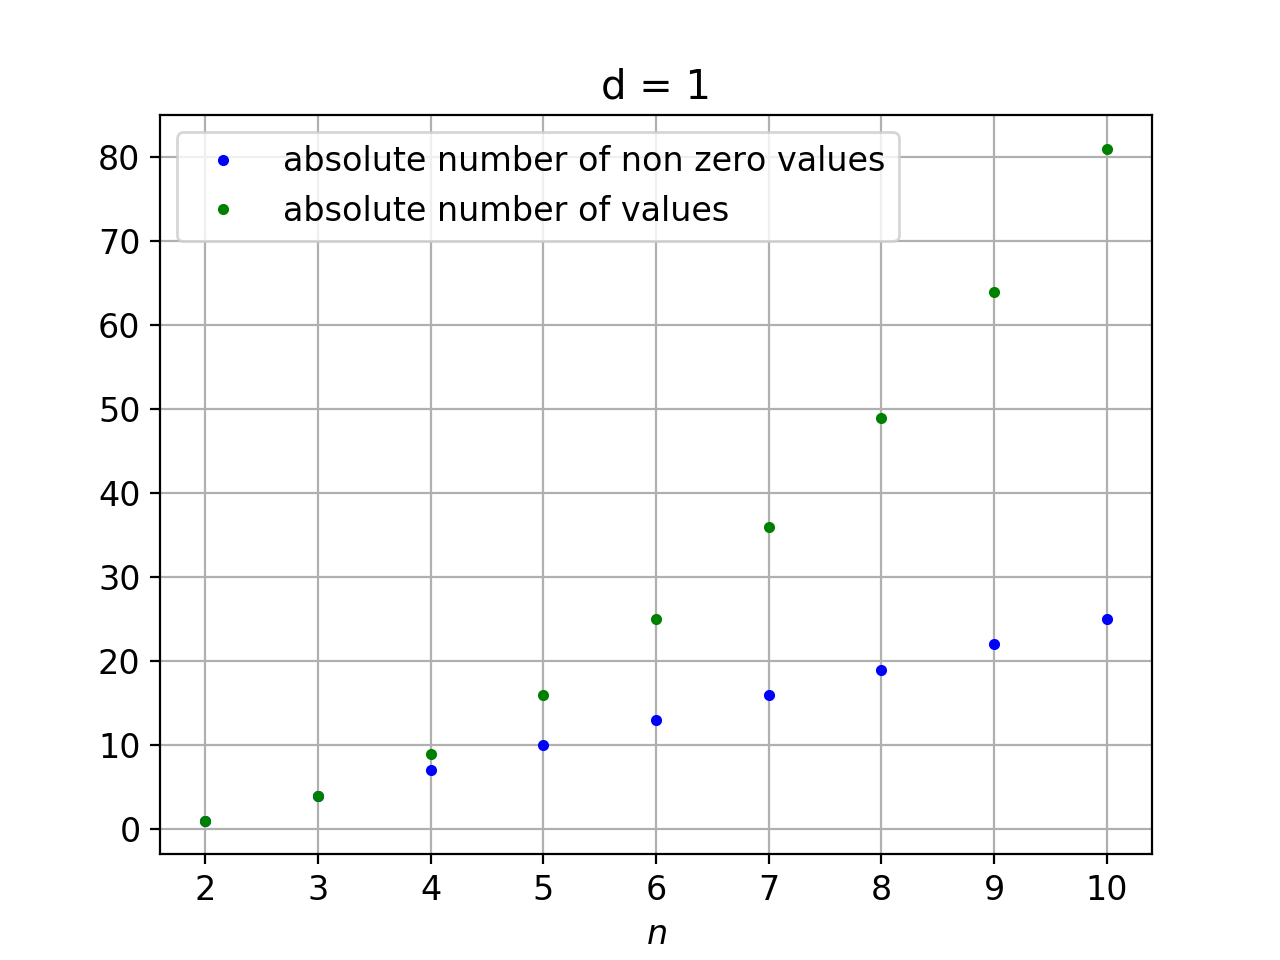
\includegraphics[width=0.6\textwidth]{Figure_1}
    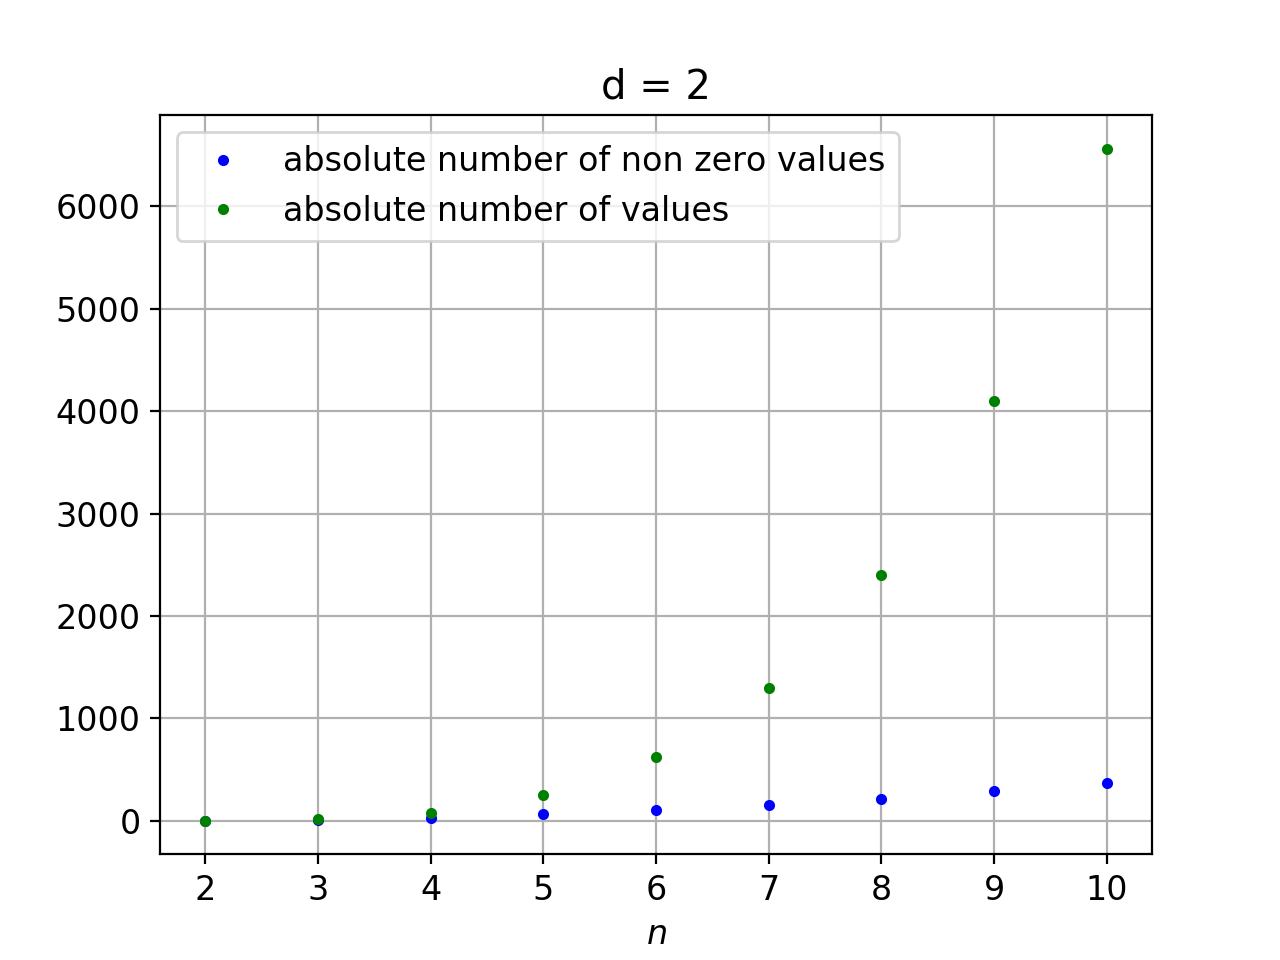
\includegraphics[width=0.6\textwidth]{Figure_2}
    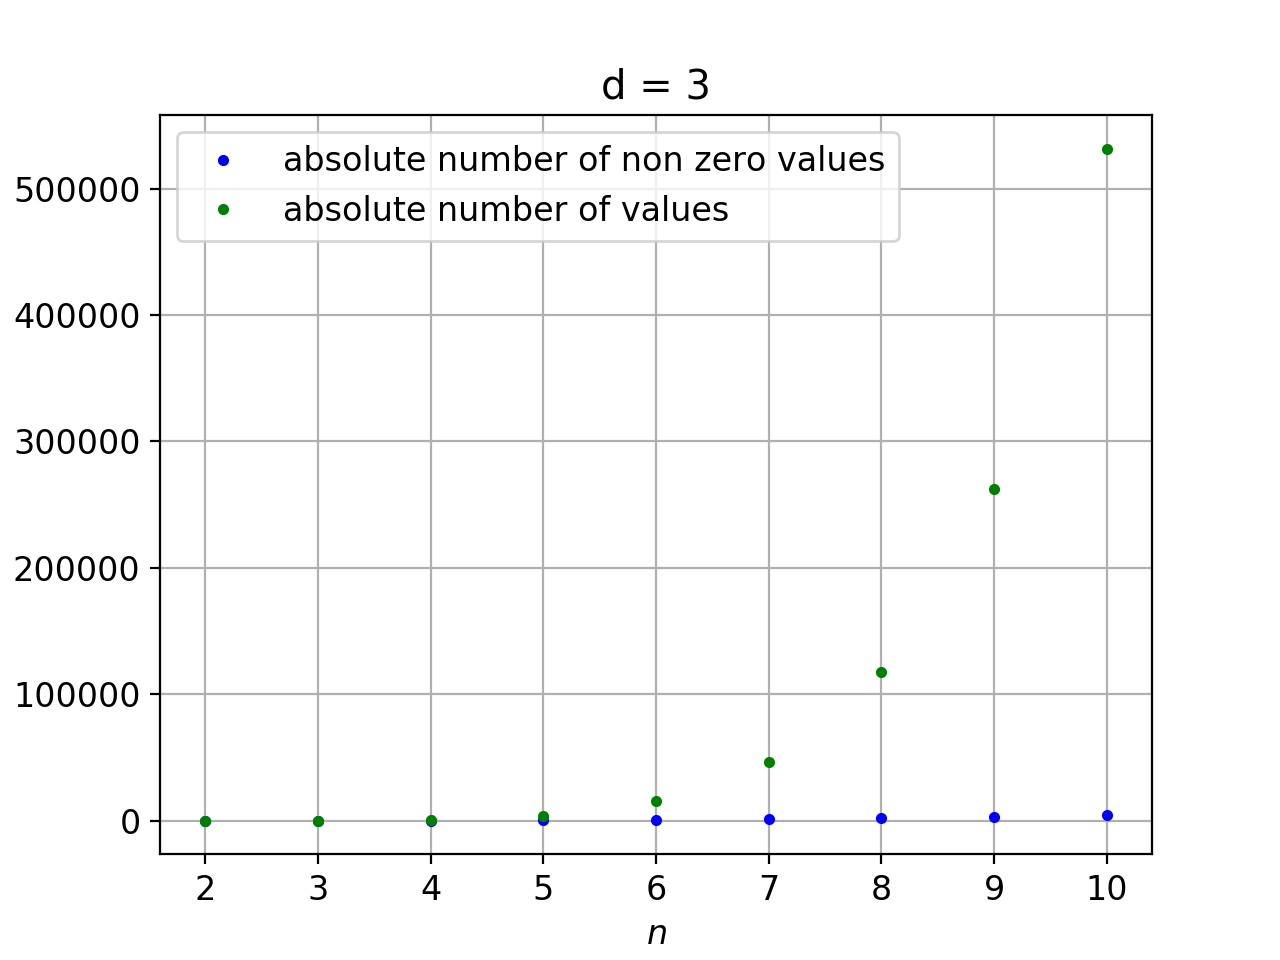
\includegraphics[width=0.6\textwidth]{Figure_3}
    \vspace{-0.2cm}
    \captionof{figure}{Anzahl von Gesamteinträgen der Matrix und der nicht-Null-Einträge für $d\in\{1, 2, 3\}$}
}
\vspace{0.5cm}

Das \textit{sparse}-Format muss zwar für jeden nicht-Null-Eintrag der Matrix bis zu drei Werte speichern, während bei einer vollbesetzten Matrix nur der Eintrag selbst gespeichert wird, jedoch kann dies trotzdem zu einer Speicherersparnis führen, wenn weniger als ein Drittel der Einträge der Matrix ungleich Null sind.
Für $d=1$ ist dies ab $n=10$ zu beobachten, wenn die vollbesetzte Matrix 81 Einträge hat, wovon aber nur 25 nicht Null sind. Für höhere $d$ tritt dieser Fall noch früher ein. Bei $d=2$ sind es schon bei $n=5$ nur noch 64 nicht-Null-Einträge in einer Matrix mit insgesamt 256 Einträgen und bei $d=3$ enthält schon bei $n=4$ die Matrix mit 19683 Einträgen nur noch 135 nicht-Null-Einträge.
Demzufolge sollte man für sehr große $d$ und $n$, die insbesondere durch das Streben nach einer besseren Genauigkeit unserer numerischen Lösung auftreten, das günstige \textit{sparse}-Format der Matrix nutzen.

\pagebreak
\section{Zusammenfassung und Ausblick}
Im Rahmen dieser Arbeit haben wir das Poisson-Problem vorgestellt und einen Lösungsansatz aufgezeigt.
Dabei haben wir es mittels einer Diskretisierung des Gebietes und des Laplace-Operators in das Lösen eines linearen Gleichungssystem überführt, das eine spezielle Struktur aufweist, die bei der Entwicklung eines schnellen Lösungsalgorithmus ausgenutzt werden kann.
Da es bei Prolemen in der Praxis, die mit einer hinreichend großen Genauigkeit gelöst werden sollen, zu einer sehr großen Anzahl von zu lösenden Gleichungen kommt, kann an dieser Stelle nicht per Hand verfahren werden -- eine Maschine muss übernehmen.\\
Wir haben demonstriert, dass das Speicherformat der \textit{sparse}-Matrizen sinnvoll ist, um den Aufwand hinsichtlich des Speicherplatzbedarfes bei der Lösung des Poisson-Problem mittels Finite-Differenzen-Diskretisierung gering zu halten.
Denn die Matrizen des aufgestellten linearen Gleichungssystems sind nur dünn besetzt, weisen also eine Vielzahl an Null-Einträgen auf.\\
Wie man schließlich lineare Gleichungssysteme mit dem Computer lösen kann, wollen wir in den nächsten Berichten untersuchen.
Hierbei werden wir sowohl direkte als auch iterative Verfahren beleuchten.

\pagebreak

\bibliographystyle{plain}
\bibliography{serie2_literatur}

\end{document}